\chapter{Theoretical Shenanigans}

\begin{theorem}[Couto et al.\cite{couto2011exact}]
When given a polygon $P$ and a guard set $G$, a subset $G_{sub}$ of $G$ fully covers $P$ if and only if it covers all witnesses in the shadow witness set $W$ of $G$.
\end{theorem}
\begin{proof}
The necessity condition follows trivially from $W\subset P$. As for the sufficiency condition, consider the largest area $R$ that is not covered by $G_{sub}$. Because of the atomicity of AVPs, $R$ must consist of one or more AVPs. Now consider the AVP $f$ with minimal guard subset $G_{f}$ in $R$. We show that $f$ must be a shadow AVP, a contradiction. If $f = R$, then $f$ trivially must be a shadow AVP. Otherwise, consider the neighbors of $f$. For all neighbors in $R$, $G_{f}$ can not contain their guard subset as $G_{f}$ is minimal in R. As for the neighbors not in $R$, if there exists a neighbor of which the guard subset is contained in $G_{f}$, then $f$ must be covered by one of the guards in that subset and can not be part of $R$. Otherwise, $G_{f}$ does not contain any of its neighbors' guard subsets and thus is a shadow AVP.
\end{proof}

\begin{theorem}
When given a polygon $P$ and a guard set $G$, the guard subsets of a light polygon form a clique in the 2-link-visibility graph $G_{vis}$ of $G$, and the cliques of all light polygons cover all edges of the graph.
\end{theorem}
\begin{proof}
The guard subset of a light polygon is formed by all the guards whose visibility polygons intersect in it, thus trivially forming a clique in $G_{vis}$. Assuming that for $g,g'\in G$ there exists an edge $(g, g')$ in $G_{vis}$ that is not covered by those cliques, then there exists an AVP $f$ that is not light and contains $g$ and $g'$ in its guard subset $G_{sub}$. As $f$ is not light there exists a neighboring AVP $f'$ whose guard subset contains $G_{sub}$. One can continue this argument with $f'$, but as the number of AVPs is finite, we will eventually reach an AVP $f^{*}$ of which the guard subset is not contained in its neighbors. Thus, $f^{*}$ is a light AVP and contains $g$ and $g'$, a contradiction.
\end{proof}

\begin{figure}[htbp]
\centering
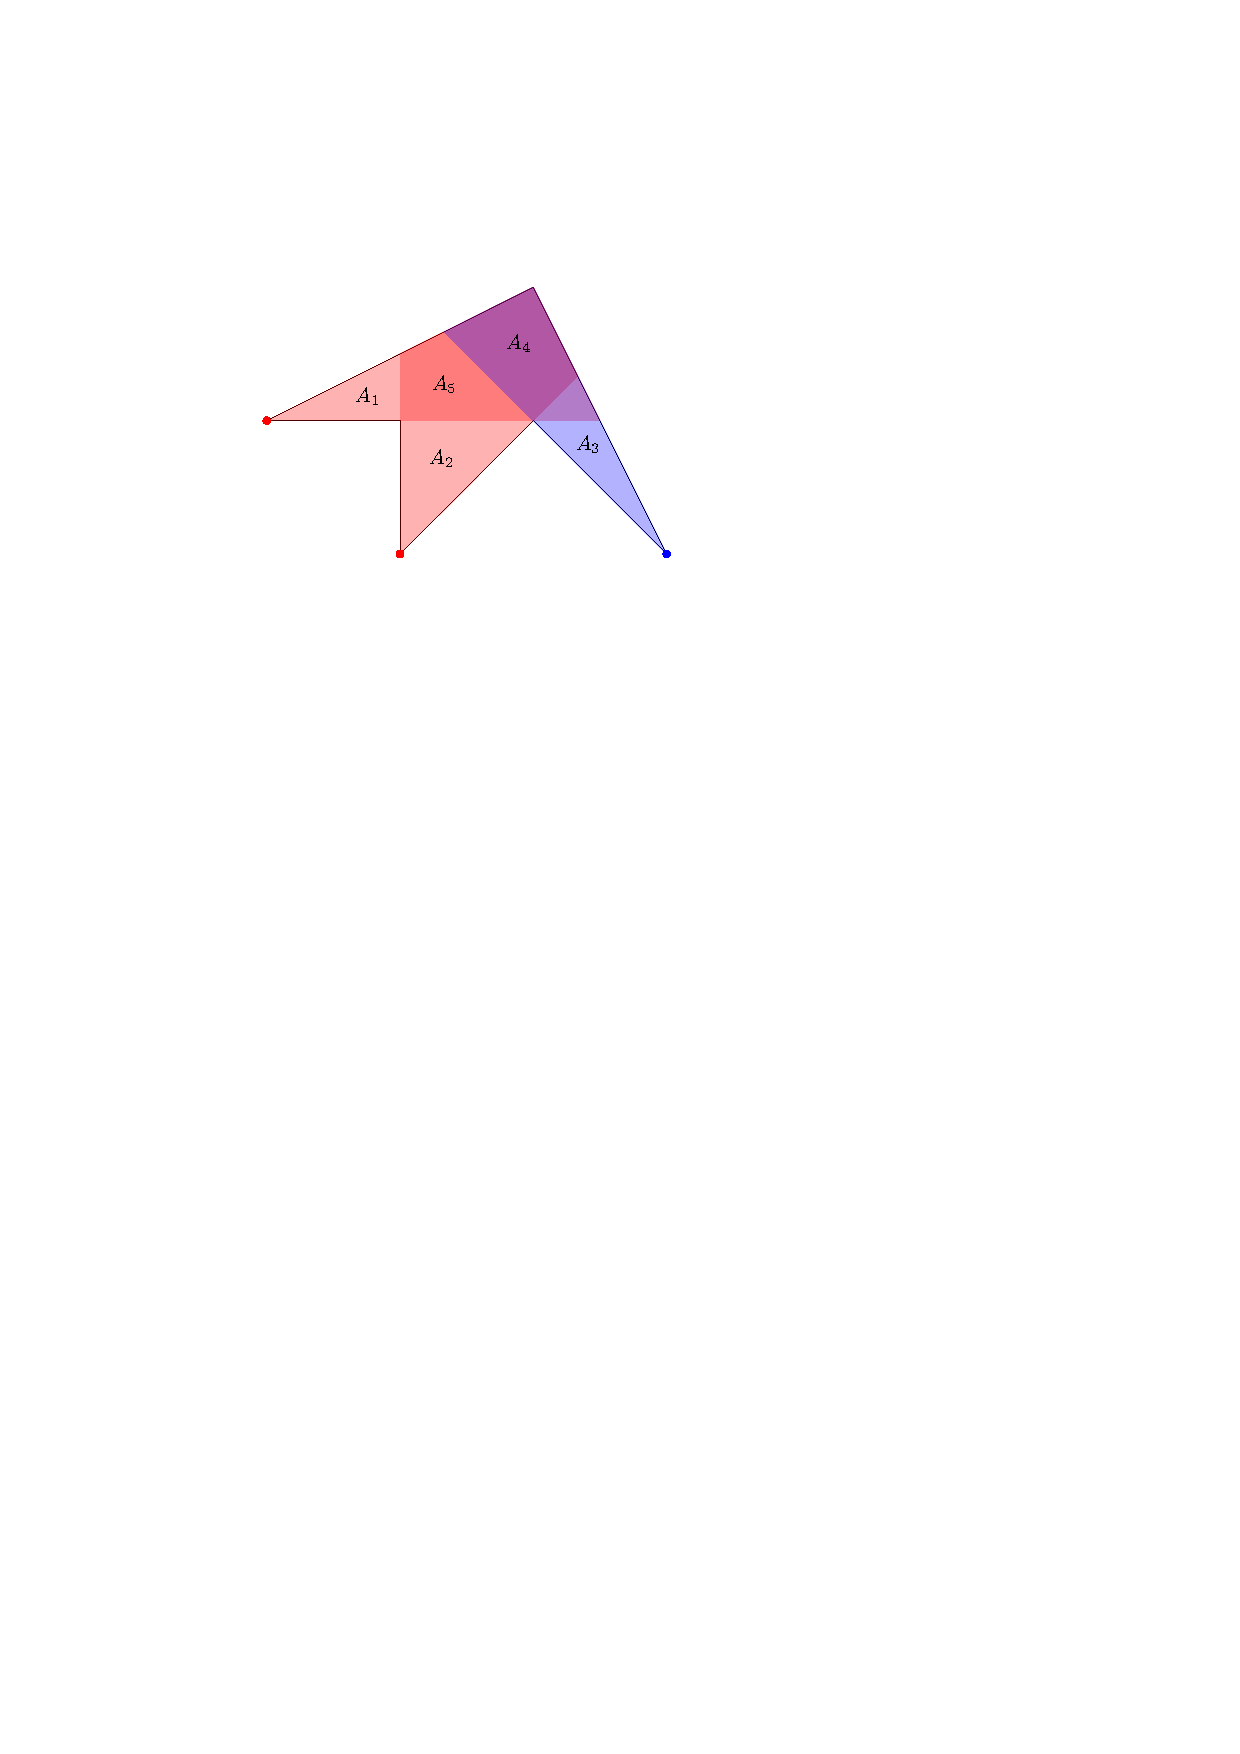
\includegraphics[scale=1.3]{Thesis/figures/conflict-free_witnesses.pdf}
\caption{Illustration for the proof of \cref{thm:light_covers}.}
\label{fig:light_covers}
\end{figure}

\begin{theorem}\label{thm:light_covers}
For a polygon $P$ and a guard set $G$, neither conflict-freeness of all shadow witnesses nor all light witnesses guarantees conflict-freeness within all AVPs.
\end{theorem}
\begin{proof}
To prove this theorem, we present a simple example in \cref{fig:light_covers}. In the figure $A_{1}$, $A_{2}$ and $A_{3}$ are shadow AVPs and $A_{4}$ is a light AVP. Each of them is covered by a guard of unique color. On the other hand, $A_{5}$ is neither shadow nor light and is covered by two guards of the same color, thus, it is not conflict-free.
\end{proof}

\chapter{Chromatic Art Gallery Problem Formulations}

In the following sections, we introduce a MIP, a SAT, and a CPSAT formulation of the Chromatic Art Gallery Problem. The MIP formulation is the one proposed by de Souza et al. \cite{zambon2014exact}, which gets modified and turned into a SAT formula for the SAT and the CPSAT formulation.

\section{MIP Formulation}

\begin{align}
\label{eq_MIP:f.0} \mbox{minimize}~& \;\sum_{k\in \{1,...,K\}} c_{k}& \\
\label{eq_MIP:f.1} \mbox{s.t. } &\sum_{g \in H}x_{gk} <= c_{k} & \forall H \in \mathcal{H}, \forall k\in \{1,...,K\}\\
\label{eq_MIP:f.2}&\sum_{g\in N(w), k\in \{1,...,K\}}x_{gk}>=1 & \forall w\in W\\
\label{eq_MIP:f.3}&\sum_{k\in \{1,...,K\}}x_{gk}<=1 & \forall g\in G\\
\label{eq_MIP:f.4}&c_{k} - c_{k+1} >= 0 & \forall k\in \{1,...,K-1\}\\
\label{eq_MIP:f.5}&\sum_{g\in G}x_{gk} - \sum_{g\in G}x_{g(k+1)} >= 0 & \forall k\in \{1,...,K-1\}\\
\label{eq_MIP:f.6}& x_{gk} \in \{0,1\} & \forall g\in G, \forall k\in \{1,...,K\}\\
\label{eq_MIP:f.7}& c_{k}\in \{0,1\} & \forall k\in \{1,...,K\}
\end{align}

The MIP formulation of the problem introduces binary variables for every guard color combination \cref{eq_MIP:f.6} and every color \cref{eq_MIP:f.7}. The guard color variables are true whenever the guard is used and is assigned the associated color in the solution. The color variables are true whenever a guard uses that color in a solution. The objective function \cref{eq_MIP:f.0} minimizes the number of colors used in the solution. The constraints in \cref{eq_MIP:f.1} are called edge clique cover constraints. They ensure that for every clique in an edge clique cover of the 2-link-visibilty-graph $G_{vis}$ and every color only one of the guards in that clique can be assigned that color. At the same time, they make sure that if a guard in that clique uses the color, the corresponding color variable must also be true. How to find an edge clique cover for $G_{vis}$, will be discussed in the Implementation Details chapter. The constraints in \cref{eq_MIP:f.2} are called witness covering constraints. They ensure that for every witness in the witness covering graph $G_{cov}$ at least one guard in its neighborhood is used in the solution, thus the witness gets covered. We call the constraints in \cref{eq_MIP:f.3} guard coloring constraints. They ensure that each guard is assigned at most one color. Technically, these constraints are not necessary to find an optimal solution, as one can simply process the solution by deciding on one color for every guard that got assigned multiple. The reason for still including these constraints is that they reduce the space of possible optimal and near-optimal solutions, which can help the solver arrive at an optimal solution faster. In the same mindset, we add the constraints \cref{eq_MIP:f.4} and \cref{eq_MIP:f.5}, which are symmetry breaker constraints. \cref{eq_MIP:f.4} ensure that when $k$ colors are used, those colors are the first k colors in $\{1,...,K\}$. As for \cref{eq_MIP:f.4}, they induce a partial order of the colors over the size of guards using that color. This reduces the possible permutations of the colors assigned to each guard in an optimal solution.

\section{SAT Formulation}

\begin{align}
\label{eq_SAT:f.0}&\lnot x_{uk} \lor \lnot x_{vk} & \forall (u,v)\in E_{G}, \forall k\in \{1,...,K\}\\
\label{eq_SAT:f.1}&\bigvee_{g\in N(w), k\in \{1,...,K\}}x_{gk} & \forall w\in W\\
\label{eq_SAT:f.2}&\bigwedge_{1 \leq i < j \leq K} (\lnot x_{gi} \lor \lnot x_{gj}) & \forall g\in G\\
\label{eq:_SATf.3}& x_{gk} \in \{0,1\} & \forall g\in G, \forall k\in \{1,...,K\}
\end{align}

The SAT formulation of the problem differs from the MIP formulation in the way that we are not trying to minimize the number of colors used. Instead, we test whether there exists a feasible solution given a fixed number of colors K. By doing so, we can solve the SAT formula for different numbers of colors, increasing the number whenever we encounter infeasibility and decreasing it on a feasible solution, until we find the smallest number of colors for which there exists a feasible solution. The exact procedure for choosing the number of colors will be discussed in the Implementation Details chapter. Because we have a fixed number of colors, we do not require color variables like \cref{eq_MIP:f.7} anymore and restrict ourselves to the guard color variables in \cref{eq:_SATf.3}. We also omit the symmetry breaker constraints \cref{eq_MIP:f.4} and \cref{eq_MIP:f.5}, as \cref{eq_MIP:f.4} uses color variables and we found no straightforward way to model them efficiently using SAT clauses. Now for the clauses in our SAT formulation, we ensure that no two guards that share an edge in the 2-link-visibility graph $G_{vis}$ share the same color using \cref{eq_SAT:f.0}. These clauses replace the edge clique cover constraints in \cref{eq_MIP:f.1}. The reason for simply using the edges of $G_{vis}$ and not cliques is that SAT solvers are very efficient at solving large numbers of small clauses i.e. with only two variables. For the witness covering constraints \cref{eq_MIP:f.2}, we use the clauses in \cref{eq_MIP:f.1}, which have an equivalent meaning. Lastly, we use the clauses in \cref{eq_MIP:f.2} to replace the guard coloring constraints in \cref{eq_MIP:f.3}. Again, these constraints can be omitted by processing the solution at the end and we will compare the performance with and without them in the Experiments chapter below.

\section{CPSAT Formulation}

As CPSAT solvers allow for both MIP and SAT constraints, we use both the MIP and the SAT formulation and compare them against each other in the Experiments chapter.

\chapter{Conflict-free Chromatic Art Gallery Problem Formulations}

In the following sections, we introduce a MIP, a SAT, and a CPSAT formulation of the Conflict-free Chromatic Art Gallery Problem.

\section{MIP Formulation}

\begin{align}
\label{eq_MIP_cf:f.0} \mbox{minimize}~& \;\sum_{k\in \{1,...,K\}} c_{k}& \\
\label{eq_MIP_cf:f.1} \mbox{s.t. } &\sum_{g \in G}x_{gk} >= c_{k} & \forall k\in \{1,...,K\}\\
\label{eq_MIP_cf:f.2}&\sum_{g\in G}x_{gk} <= |G|\cdot  c_{k} & \forall k\in \{1,...,K\}\\
\label{eq_MIP_cf:f.3}&\sum_{g\in N(w)}x_{gk} >= u_{wk} & \forall w\in W, \forall k\in \{1,...,K\}\\
\label{eq_MIP_cf:f.4}&\sum_{g\in N(w)}x_{gk} <= 1 + |N(w)|\cdot  (1-u_{wk}) & \forall w\in W, \forall k\in \{1,...,K\}\\
\label{eq_MIP_cf:f.5}&\sum_{k\in \{1,...,K\}}u_{wk} >= 1 & \forall w\in W\\
\label{eq_MIP_cf:f.6}&\sum_{k\in \{1,...,K\}}x_{gk} <= 1 & \forall g\in G\\
\label{eq_MIP_cf:f.7}&c_{k} - c_{k+1} >= 0 & \forall k\in \{1,...,K-1\}\\
\label{eq_MIP_cf:f.8}&\sum_{g\in G}x_{gk} - \sum_{g\in G}x_{g(k+1)} >= 0 & \forall k\in \{1,...,K-1\}\\
\label{eq_MIP_cf:f.10}& u_{wk} \in \{0,1\} & \forall w\in W, \forall k\in \{1,...,K\}\\
\label{eq_MIP_cf:f.11}& x_{gk} \in \{0,1\} & \forall g\in G, \forall k\in \{1,...,K\}\\
\label{eq_MIP_cf:f.12}& c_{k}\in \{0,1\} & \forall k\in \{1,...,K\}
\end{align}

The MIP formulation for the CCAGP is similar to the one of the CAGP. We are still trying to minimize the number of colors \cref{eq_MIP_cf:f.0} and keep the same variables \cref{eq_MIP_cf:f.11} for colors and \cref{eq_MIP_cf:f.12} for guard color combinations. Additionally, we add auxiliary variables \cref{eq_MIP_cf:f.10}, called unique color witness variables, for all witness color combinations. They are true whenever there exists exactly one guard with that color in the neighborhood of that witness. To ensure that the color variables are true if and only if a guard variable of that color is true, we add the constraints in \cref{eq_MIP_cf:f.1} and \cref{eq_MIP_cf:f.2}. The constraints \cref{eq_MIP_cf:f.3} and \cref{eq_MIP_cf:f.4} ensure that if a unique color witness variable is true, exactly one guard in the neighborhood of that witness has that color. Otherwise, there can be arbitrarily many guards of that color in the neighborhood. Lastly, we keep the guard coloring constraints \cref{eq_MIP_cf:f.6} and symmetry breaker constraints \cref{eq_MIP_cf:f.7} and \cref{eq_MIP_cf:f.8} of the CAGP MIP Formulation.

\section{SAT Formulation}

\begin{align}
\label{eq_SAT_cf:f.0}&\lnot u_{wk} \lor \bigvee_{g \in N(w)}x_{gk} & \forall w \in W, \forall k\in \{1,...,K\}\\
\label{eq_SAT_cf:f.1}&\bigwedge_{(i,j)\in {G\choose 2}} (\lnot u_{wk} \lor \lnot x_{ik} \lor \lnot x_{jk}) & \forall w \in W, \forall k\in \{1,...,K\}\\
\label{eq_SAT_cf:f.2}&\bigvee_{k\in \{1,...,K\}}u_{wk} & \forall w\in W\\
\label{eq_SAT_cf:f.3}&\bigwedge_{1 \leq i < j \leq K} (\lnot x_{gi} \lor \lnot x_{gj}) & \forall g\in G\\
\label{eq_SAT_cf:f.4}& u_{wk} \in \{0,1\} & \forall w\in W, \forall k\in \{1,...,K\}\\
\label{eq_SAT_cf:f.5}& x_{gk} \in \{0,1\} & \forall g\in G, \forall k\in \{1,...,K\}
\end{align}

For the SAT formulation of the CCAGP, we test the feasibility of the SAT formula for a fixed K in the same fashion as for the CAGP, until we find a feasible solution with a minimal number of colors. We again omit the color variables and keep the unique color witness variables \cref{eq_SAT_cf:f.4} and guard color variables \cref{eq_SAT_cf:f.5}. The clauses \cref{eq_SAT_cf:f.0} are equivalent to the constraints in \cref{eq_MIP_cf:f.3}. For all witness color combinations, if the unique color witness variable of that color and that witness is true, at least one guard of the color in the neighborhood of that witness has to be true. The clauses \cref{eq_SAT_cf:f.1} are equivalent to the constraints in \cref{eq_MIP_cf:f.4}. For all witness color combinations, if the unique color witness variable of that color and that witness is true, no two guards in the neighborhood of that witness can have that color. As for \cref{eq_SAT_cf:f.2}, these clauses represent the constraints in \cref{eq_MIP_cf:f.5}. Lastly, the witness coloring constraints \cref{eq_SAT_cf:f.3} are modeled using the same clauses as in the CAGP SAT Formulation.

\section{CPSAT Formulation}
Similar to the Chromatic Art Gallery Problem, we use both the MIP and the SAT formulation for CPSAT and compare them against each other in the Experiments chapter.

\chapter{Implementation Details}

\section{Instance Processing}
The instances are given as lists of points, which represent the outer boundaries of the polygons and possible holes. First, we create a CGAL Polygon\_with\_holes\_2 using the instance input. Then, using the vertices of the polygon and its holes as the guard set $G$, we calculate the visibility regions as polygons for each guard using CGAL's "Triangular\_expansion\_visibility\_2.h" and save each guard together with its visibility polygon in a list. Afterward, we recursively overlay the visibility polygons using CGAL's "Arr\_overlay\_2.h" to obtain the AVP arrangement (\cref{alg:AVP_generation}). To be able to form the partial order over the AVPs, we overload the overlay function to save for every face a set of guards from which it was created. 

\begin{algorithm}
\caption{generate\_AVP\_recursive(guards: list[tuple[int, Polygon\_with\_holes\_2]])}\label{alg:AVP_generation}
\begin{algorithmic}
\STATE $half\gets len(guards)/2$
\STATE $firstHalf\gets guards[:half]$ 
\STATE $secondHalf\gets guards[half:]$
\IF{$len(guards) = 1$}
    \STATE $Arrangement(guards[0][0], guards[0][1])$
\ELSE
    \STATE $generate\_AVP\_recursive(firstHalf).overlay(generate\_AVP\_recursive(secondHalf))$
\ENDIF
\end{algorithmic}
\end{algorithm}

For the CAGP, we calculate the shadow witness set. As geometric operations are expensive, instead of saving the shadow witness set as a set of points, we store each witness as an integer together with the set of guards that covers the witness as well as each guard together with the set of witnesses that the guard covers. Additionally, we store a list of the set of guards for each light AVP. For the CCAGP, we calculate the witness set as well. But because of \cref{thm:light_covers} just using shadow or light witnesses is not sufficient, thus we use a witness for every AVP instead. 

\begin{algorithm}
\caption{Calculate witness sets and light guard sets}
\begin{algorithmic}[1]
\STATE Initialize empty maps:\\ $witness\_to\_guards,\linebreak guard\_to\_witnesses,\linebreak all\_witness\_to\_guards,\linebreak all\_guard\_to\_witnesses$
\STATE Initialize empty list:\\ $light\_guard\_sets$
\STATE $shadow\_index\gets 0$
\STATE $all\_index\gets 0$
\FORALL{face in faces}
    \STATE $g\_data\gets$ guard set of the face
    \IF{$g\_data$ is empty}
        \STATE Continue
    \ENDIF
    \STATE $is\_shadow\gets \TRUE$
    \STATE $is\_light\gets \TRUE$
    \FORALL{half\_edge in face}
        \STATE $twin\_g\_data\gets$ guard set of the twin face of the half\_edge
        \IF{$twin\_g\_data$ is empty}
            \STATE Continue
        \ENDIF
        \IF{$g\_data\subset twin\_g\_data$}
            \STATE $is\_shadow\gets \FALSE$
        \ENDIF
        \IF{$twin\_g\_data\subset g\_data$}
            \STATE $is\_light\gets \FALSE$
        \ENDIF
    \ENDFOR
    \STATE $all\_witness\_to\_guards[all\_index]\gets g\_data$
    \FORALL{$g$ in $g\_data$}
        \STATE $all\_guard\_to\_witnesses[g]\gets all\_guard\_to\_witnesses[g]\cup all\_index$
    \ENDFOR
    \STATE $all\_index\gets all\_index + 1$
    \IF{$is\_shadow$}
        \STATE $witness\_to\_guards[index]\gets g\_data$
        \FORALL{$g$ in $g\_data$}
            \STATE $guard\_to\_witnesses[g]\gets guard\_to\_witnesses[g]\cup index$
        \ENDFOR
        \STATE $shadow\_index\gets shadow\_index + 1$
    \ENDIF
    \IF{$is\_light$}
        \STATE $light\_guard\_sets.insert(g\_data)$
    \ENDIF
\ENDFOR
\RETURN\linebreak $witness\_to\_guards,\linebreak guard\_to\_witnesses,\linebreak light\_guard\_sets,\linebreak all\_witness\_to\_guards,\linebreak all\_guard\_to\_witnesses$
\end{algorithmic}
\end{algorithm}

\section{Initial Upper Bound}
Calculating a low initial upper bound is vital for efficiently solving the CAGP and CCAGP, as the possible number of colors K directly affects the size of the problem formulation. To achieve this, we implement the approach presented by de Souza et al. \cite{zambon2014exact}, for which K was on average only 1.7 larger than the number of colors used by the optimal solution. 

\section{Edge Clique Covers}

\section{Lazy Constraints}

\section{SAT color optimization}